\documentclass[letterpaper]{article}
\usepackage[utf8]{inputenc}
\usepackage[T1]{fontenc}
\usepackage[activeacute,spanish]{babel}
\usepackage[vmargin=4cm,tmargin=3cm,hmargin=2cm,letterpaper]{geometry}%
\usepackage{helvet}
\usepackage{amsmath,amsfonts,amssymb}
\newtheorem{prop}{Proposción}
\newtheorem{prue}{Prueba}
\usepackage{graphicx}
\usepackage{caption}
\usepackage{subcaption}
\usepackage{float}
\usepackage[usenames,dvipsnames]{color}
\usepackage[usenames,dvipsnames,svgnames,table]{xcolor}
\usepackage{verbatim}
\usepackage{tabls}
\usepackage{lastpage}
\usepackage{fancyhdr}
\usepackage{url}
\usepackage{listings}
%%%%%%%%%%%%%%%%%%%%%%%%%%%%%%%%%%%%%%%%%%%%%%%%%%%%%%%%%%%%%%%%%%%%%%%%%%%%%%%%%%%%%%%
%\usepackage{tikz}
\usepackage{pgf}
\usepackage{pgffor}
\usepgfmodule{plot}
\usepackage{wrapfig}
\usepackage{algpseudocode}
\usepackage{algorithm}
%\usetikzlibrary{arrows,decorations,snakes,backgrounds,fit,calc,through,scopes,positioning,automata,chains,er,fadings,calendar,matrix,mindmap,folding,patterns,petri,plothandlers,plotmarks,shadows,shapes,shapes.arrows,topaths,trees}


%------------------------------------------------configuración de lisnting para código de C
\usepackage{listings}	% Para códigos: C, C++, python
\usepackage[usenames,dvipsnames]{color}% Para gama de colores ver http://en.wikibooks.org/wiki/LaTeX/Colors
\lstset{language=C, basicstyle=\color{Gray}\ttfamily\normalsize, keywordstyle=\color{RoyalBlue}\ttfamily\normalsize, stringstyle=\color{WildStrawberry}\ttfamily\normalsize, commentstyle=\color{Emerald}\ttfamily, morecomment=[l][\color{Thistle}]{\#}}
%------------------------------------------------

\lstset{% general command to set parameter(s)
%   basicstyle=\small,
  % print whole listing small
%   keywordstyle=\color{black}\bfseries\underbar,
  % underlined bold black keywords
%   identifierstyle=,
  % nothing happens
%   commentstyle=\color{white}, % white comments
%   stringstyle=\ttfamily,
  % typewriter type for strings
  showstringspaces=false}
  % no special string spaces

\pagestyle{fancy}
\color{black}
\fancyhead{}
\renewcommand{\headrule}{\hrule\vspace*{0.5mm}\rule{\linewidth}{0.8mm}}
\renewcommand{\familydefault}{\sfdefault}

\graphicspath{{./images/}}
\lhead{
\includegraphics[width=2cm]{Images/logoucr.png}}
\rhead{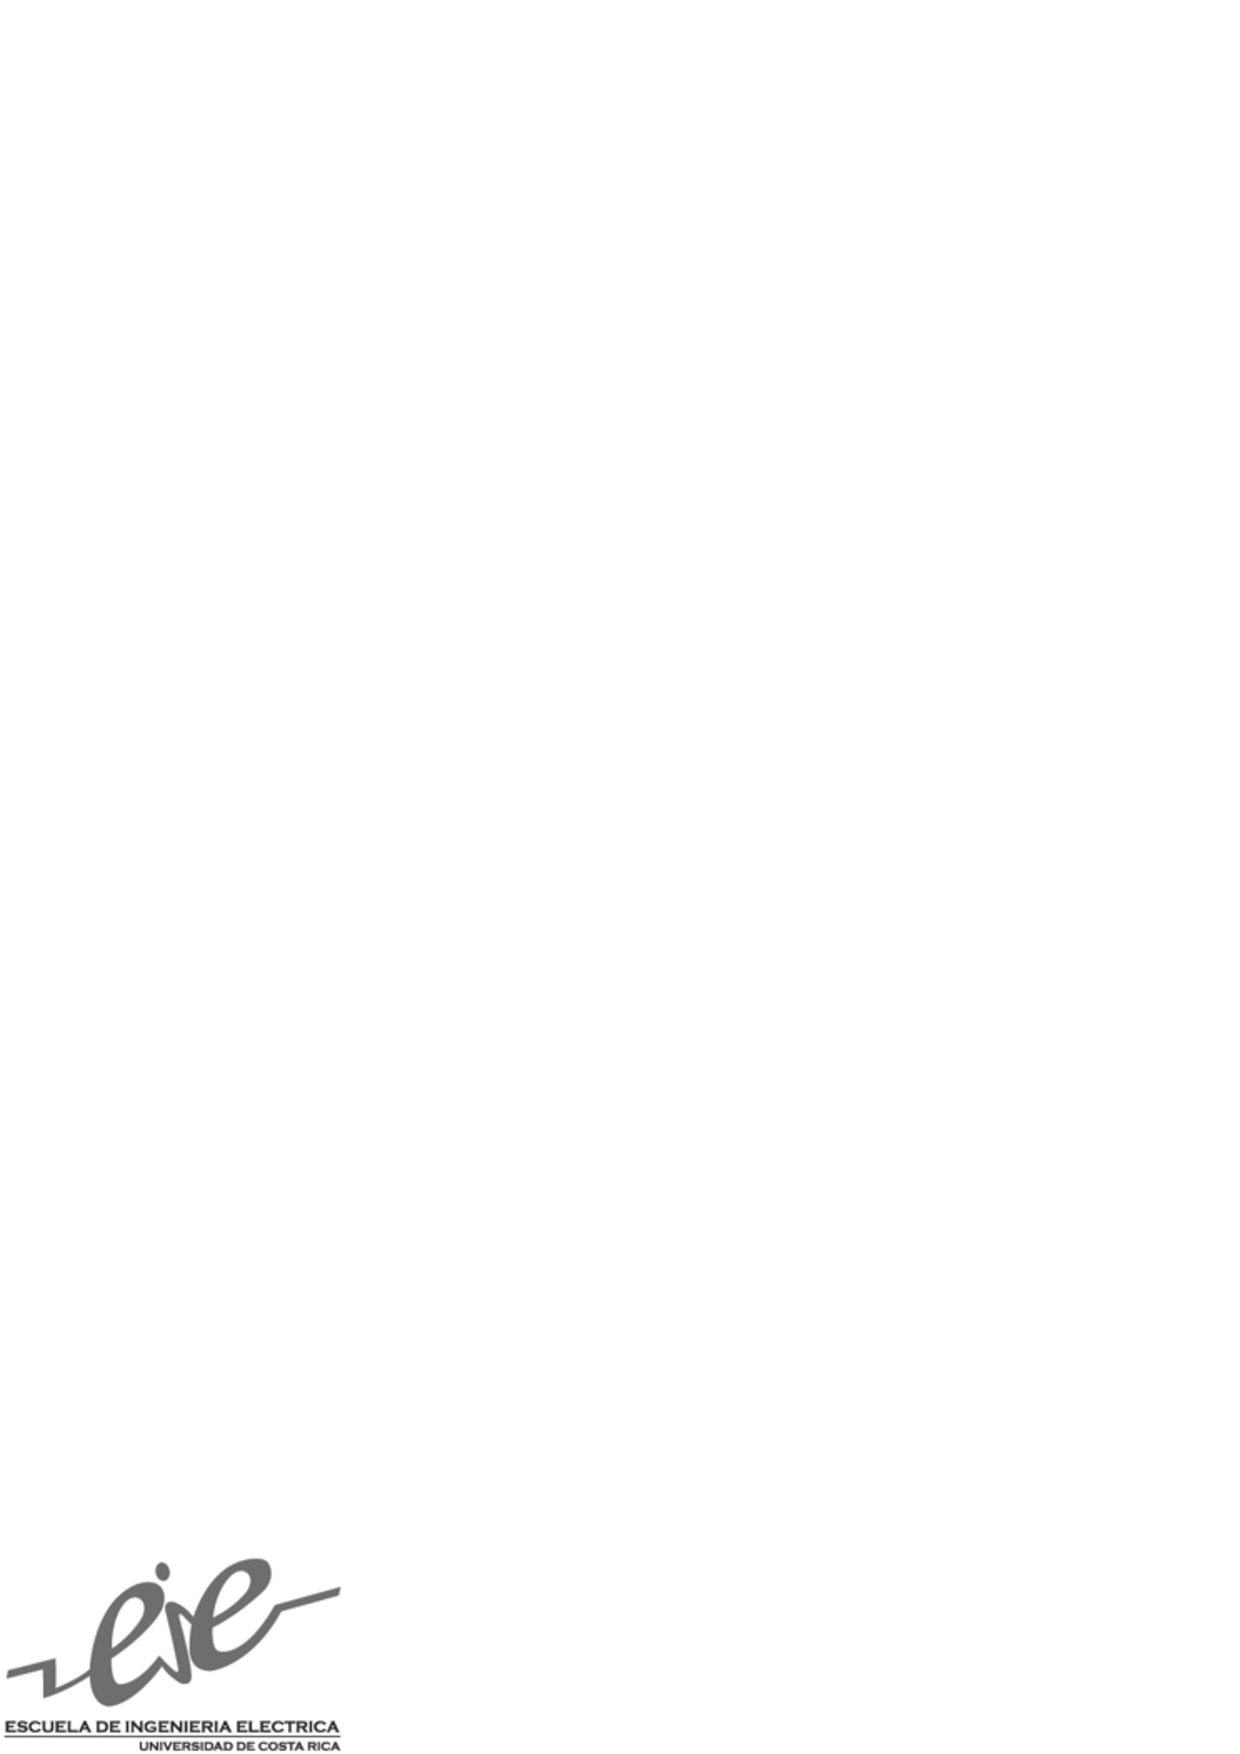
\includegraphics[width=3cm]{Images/eie-text-gray-6x3cm.png}}
\chead{UNIVERSIDAD DE COSTA RICA\\FACULTAD DE INGENIERÍA\\ESCUELA DE INGENIERÍA ELÉCTRICA\\\textbf{ESTRUCTURAS ABSTRACTAS DE DATOS Y\\ ALGORITMOS PARA INGENIERÍA}\\IE-0217\\I CICLO 2011\\INVESTIGACIÓN BIBLIOGRÁFICA 2}

\lfoot{}%
\cfoot{}%
%\cfoot{\thepage\ de \pageref{LastPage}}%
\rfoot{}%

%%%%%%%%%%%%%%%%%%%%%%%%%%%%%%%%%%%%%%%%%%%%%%%%%%%%%%%%%%%%%%%%%%%%%%%%%%%%%%%%%%%%%%%%%%%%%%%%%%%%%%%%%%%%%%%
\newcommand{\uic}{blue} %user-input color
%%%%%%%%%%%%%%%%%%%%%%%%%%%%%%%%%%%%%%%%%%%%%%%%%%%%%%%%%%%%%%%%%%%%%%%%%%%%%%%%%%%%%%%%%%%%%%%%%%%%%%%%%%%%%%%%%%
\newcommand{\uim}{\_\_} %user-input marker
%%%%%%%%%%%%%%%%%%%%%%%%%%%%%%%%%%%%%%%%%%%%%%%%%%%%%%%%%%%%%%%%%%%%%%%%%%%%%%%%%%%%%%%%%%%%%%%%%%%%%%%%%%%%%%%%%%
\newcommand{\userinput}[1]{\textcolor{\uic}{\uim#1\uim}}


%%%%%%%%%%%%%%%%%%%%%%%%%%%%%%%%%%%%%%%%%%%%%%%%%%%%%%%%%%%%%%%%%%%%%%%%%%%%%%%%%%%%%%%%%%%%%%%%%%%%%%%%%%%%%%%%%%
\begin{document}\vspace*{2cm}
%%%%%%%%%%%%%%%%%%%%%%%%%%%%%%%%%%%%%%%%%%%%%%%%%%%%%%%%%%%%%%%%%%%%%%%%%%%%%%%%%%%%%%%%%%%%%%%%%%%%%%%%%%%%%%%%%%

%%%%%%%%%%%%%%%%%%%%%%%%%%%%%%%%%%%%%%%%%%%%%%%%%%%%%%%%%%%%%%%%%%%%%%%%%%%%%%%%%%%%%%%%%%%%%%%%%%%%%%%%%%%%%%%%%%
\begin{center}
\Huge
Colas de Prioridad en el algoritmo de Prim para grafos de aristas con peso
\vspace*{1cm}
\end{center}

\noindent
\small\baselineskip=14pt
\textbf{Estudiante:} Ernesto Céspedes Montero\\
\textbf{Carné:} A31355\\

%%%%%%%%%%%%%%%%%%%%%%%%%%%%%%%%%%%%%%%%%%%%%%%%%%%%%%%%%%%%%%%%%%%%%%%%%%%%%%%%%%%%%%%%%%%%%%%%%%%%%%%%%%%%%%%%%%
\section{Introducción}

La teoría de grafos tiene su relevancia en la gran cantidad de aplicaciones reales en las que se utilizan algoritmos de optimización de rutas. Podemos así mencionar distintas áreas en las que se aplican estos algoritmos como redes de computadoras, mapas, contenido Web, circuitos, redes sociales, etc.

	El tipo de grafos que más relevancia tiene en aplicaciones reales, son los grafos de aristas con peso (\textit{edge weighted graph}) a los cuales se les asocia un valor o peso a la arista que une dos nodos. Una aplicación relacionada con este tipo de estructura es por ejemplo la representación de las rutas de vuelo de un avión, donde los nodos representan los puntos de destino y salida, la arista representa la ruta de vuelo y a esta se le puede asignar un valor como por ejemplo la distancia a la que se encuentra la aeronave del punto de destino.
	
	Debido a esta relevancia de la teoría de grafos en aplicaciones reales, se considera importante comprender más a fondo este tipo de estructura abstracta, y en particular se ha escogido estudiar el tipo de estructura abstracta llamada cola de prioridad aplicado en el algoritmo de Prim, el cual es aplicado para hallar el árbol de expansión mínima dentro de un grafo de aristas con peso.
%%%%%%%%%%%%%%%%%%%%%%%%%%%%%%%%%%%%%%%%%%%%%%%%%%%%%%%%%%%%%%%%%%%%%%%%%%%%%%%%%%%%%%%%%%%%%%%%%%%%%%%%%%%%%%%%%%
\section{Objetivos}

\subsection{Objetivo General}

Comprender el uso de las colas de prioridad en el algoritmo de Prim para grafos de aristas con peso

\subsection{Objetivos Específicos}

Los objetivos específicos son:\\

\begin{enumerate}
\item Describir el concepto de la estructura abstracta de cola de prioridad
\item Mostrar la implementación de las colas de prioridad en lenguaje C++
\item Implementar el algoritmo de Prim en lenguaje de alto nivel usando colas de prioridad
\item Buscar comparaciones de eficiencia del algoritmo de Prim, al usar colas de Prioridad contra el uso de otro tipo de estructuras como \textit{heaps}
\end{enumerate}

%%%%%%%%%%%%%%%%%%%%%%%%%%%%%%%%%%%%%%%%%%%%%%%%%%%%%%%%%%%%%%%%%%%%%%%%%%%%%%%%%%%%%%%%%%%%%%%%%%%%%%%%%%%%%%%%%%
\section{Metodología}

La metodología implementada en esta trabajo se basó en la investigación bibliográfica del algoritmo seleccionado utilizando fuentes primarias como libros de introducción a algoritmos y estructuras de datos en lenguajes de alto nivel. Específicamente se consultó material referente a estructuras de datos básicas de datos como trees, binary heap's, stack's, bag's, queue's y finalmente priority queue's. Esta última estructura fué ampliamente investigada pues es la base de obtención del árbol de expansión mínima en un grafo de aristas con peso, usando el algoritmo de Prim.

Consultando otras fuentes se encontró teoría de procesamiento de grafos con peso y específicamente se obtuvo el pseudocódigo del algortimo de Prim, el cual fué fácil de implementar en lenguaje C++, una vez comprendida su representación abstracta usando listas de adjayencia y colas de prioridad.

Como parte del análisis comparativo del algoritmo se estudió la diferencia de eficiencia de tiempo de ejecución cuando las colas de prioridad se implementan con heap's y cuando se hace mediante arreglos.

%%%%%%%%%%%%%%%%%%%%%%%%%%%%%%%%%%%%%%%%%%%%%%%%%%%%%%%%%%%%%%%%%%%%%%%%%%%%%%%%%%%%%%%%%%%%%%%%%%%%%%%%%%%%%%%%%%
\section{Algoritmo de Prim}

El algoritmo de Prim es un algoritmo de procesamiento de grafos de aristas con peso el cual es utilizado para encontrar el arbol de expansión mínima de este grafo. Para comprender este concepto es necesario recurrir a la Figura ~\ref{fig:MSTree}

\begin{figure}[h]
\includegraphics[width=.35\textwidth]{Images/MSTree.png}
\centering
\caption{An edge-weigthed graph and its MST}
\label{fig:MSTree}
\end{figure}

Como se mencionó previamente, un grafo de aristas con peso es aquel al que se le asigna un valor o un peso a la arista que uno dos vértices, representación abstracta que tienen mucha representaciones en problemas reales. Un árbol en un grafo es un subgrafo, es decir un subconjunto de vértices conectados a través de un subconjunto de aristas de manera no cíclica, es decir que no existan más de un único camino para llegar de un vértice a cualquier otro.\\

Por otro lado un árbol de expansión es un árbol dentro de un grafo que conecta todos sus vértices, es decir que el subconjunto que representa el árbol es el mismo conjunto de vértices del grafo entero, comprendido este concepto es fácil ahora describir el concepto de árbol de expansión mínima (MST): \textit{Un árbol de expansión mínima es el conjunto de todos los vértices de un grafo junto con el subconjunto de aristas que conectan de manera no cíclica todos estos vértices y que la suma total de los pesos de estas aristas es mínima}. En diferentes fuentes bibliográficas es común encontrar un concepto más sencillo como: \textit{El árbol de expansión mínima es el árbol de expansión de un grafo tal que la suma total del peso de las aristas es mínimo}. Cabe aclarar que el concepto de un MST solo tiene sentido para grafos de arista con peso.\\

Sin embargo para el concepto de árbol de expansión mínima que estamos considerando debemos asumir otras convenciones:

\begin{itemize}
\item El grafo del que se desea buscar el MST debe estar conectado. La definición que asumimos para un árbol de expansión implica que que el grafo debe tener sus vértices conectados para que exista el MST. En el caso de que un grafo se componga de dos subgrafos conectados pero sin conexión entre ellos, se deberá computar por aparte el algoritmo que encuentre el MST de cada subgrafo.
\item El peso o valor de cada arista en el grafo, puede ser de valor negativo o igual a cero, el concepto para MST que se explicó anteriormente de suma mínima de pesos de un árbol de expansión no se viola.
\item Los pesos de las aristas deben ser todos diferentes para que el árbol de expansión mínima sea único, de lo contrario podrán encontrarse varias soluciones al MST.
\end{itemize}

Estas consideraciones de muestran a continuación en la Figura ~\ref{fig:conve}

\begin{figure}[h]
        \centering
        \begin{subfigure}[b]{0.3\textwidth}
                \includegraphics[width=\textwidth]{Images/conve1.png}
                \caption{grafo no conectado}
                \label{fig:conve1}
        \end{subfigure}%
        ~ %add desired spacing between images, e. g. ~, \quad, \qquad, \hfill etc.
          %(or a blank line to force the subfigure onto a new line)
        \begin{subfigure}[b]{0.3\textwidth}
                \includegraphics[width=\textwidth]{Images/conve2.png}
                \caption{aristascon peso negativo}
                \label{fig:conve2}
        \end{subfigure}
        ~ %add desired spacing between images, e. g. ~, \quad, \qquad, \hfill etc.
          %(or a blank line to force the subfigure onto a new line)
        \begin{subfigure}[b]{0.3\textwidth}
                \includegraphics[width=\textwidth]{Images/conve3.png}
                \caption{MST no único}
                \label{fig:conve3}
        \end{subfigure}
        \caption{Anomalías para el MST}\label{fig:conve}
\end{figure}

El principio en el que se basa el algoritmo de Prim es una propiedad propiedad matemática que considera partir el grafo en dos partes cruzando aristas y escogiendo la de menor peso. Esta propiedad denominada \textit{Cut Property} se presenta en la siguiente proposición:

\begin{prop}
Dado cualquier corte en un grafo de aristas con peso, la arista cruzada con el peso menor, es parte del árbol de expansión mínima
\end{prop}

\begin{figure}	
\includegraphics[width=.35\textwidth]{Images/CutProp.png}
\centering
\caption{\textit{''Cut Property''} para un grafo el MST de un grafo de aristas con peso}
\label{fig:MSTree}
\end{figure}


Comprendiendo esta propiedad resulta sencillo describir el procedimiento del algoritmo de Prim para encontrar el MST de un grafo de aristas con peso. Simplemente se parte desde visitando un vértice inicial, dividiendo el grafo entre vértices visitados y no visitados, se escoge la arista de menor peso de las aristas cruzadas por esta división (cut property) para agregarla al MST, visita el siguiente vértice y aplica al mismo criterio para las aristas cruzadas excluyendo las que ya han sido agregadas al MST.

\begin{algorithm}[h]
\caption{Algoritmo de Prim}
\label{Djikstra}
\begin{algorithmic}
\Procedure{Prim}{G}
    \State PQ = empty;
    \State MST = empty;
    \State Marked = all False;
    Visit(G,0)
    \While{(PQ isn't empty)}%
        \State e = PQ.delMin( )
        \If {e does not belong to MST} continue\EndIf
       	\State add e to MST
       	\If {e.either was not visited} visit(G,e.either)\EndIf
       	\If {e.other was not visited} visit(G,e.either)\EndIf
    \EndWhile    
\EndProcedure

\Procedure{visit}{G,v}
	\State marked[V] = True
	\State Enqueue all incident edges to v in PQ
\EndProcedure
\end{algorithmic}
\end{algorithm}

 El algoritmo utiliza tres diferentes tipos de estructuras de datos para recorrer completamente el grafo y devolver el árbol de expansión mínima, específicamente utiliza un arreglo booleano de tamaño de los vértices $\mathcal{V}$ para marcar los vértices visitados, utiliza una cola de aristas en la que almacena las aristas mínimas que forman parte del MST y utiliza una cola de mínima prioridad de aristas con peso en la que encola las aristas incidentes a un vértice visitado para ordenarlas y escoger las de menor peso. En este trabajo se describe la implementación de esta cola de prioridad mediante la estructura de datos llamada \textit{heap}.\\

El algoritmo inicia visitando un vértice cualquiera (comúnmente el 0) el cual marca como visitado y encola todas sus aristas incidentes en la cola de prioridad. En cada ciclo recursivo siguiente el algoritmo extrae de la cola de prioridad la arista de menor peso para agregarla a la cola de aristas del árbol de expansión mínima. Luego selecciona como siguiente vértice a visitar el alojado en el otro extremo de la arista mínima que forma ahora parte del MST, luego encola en la cola de prioridad las aristas incidentes al nuevo vértice visitado y se extiende a lo largo del grafo hasta que todos los vértices hayan sido marcados como visitados. Finalmente el algoritmo retorna un puntero la cola que contiene las aristas que conforman el árbol de expansión mínima deseado. El siguiente pseudocódigo anterior resume lo explicado




%%%%%%%%%%%%%%%%%%%%%%%%%%%%%%%%%%%%%%%%%%%%%%%%%%%%%%%%%%%%%%%%%%%%%%%%%%%%%%%%%%%%%%%%%%%%%%%%%%%%%%%%%%%%%%%%%%
\section{Colas de prioridad}

Una cola de prioridad en una estructura abstracta de datos que colecciona objetos y soporta básicamente dos funciones: \textit{insertar} nuevos objetos, y \textit{remover el de máxima} (ó mínima) prioridad, es decir es una estructura de datos donde estos se extraen considerando un criterio de prioridad (o valor de prioridad) e ingresan de manera aleatoria. Una cola de prioridad tiene su analogía en la vida cotidiana en los de atención de clientes bancarios por ejemplo: "no necesariamente se atienden conforme el orden en que ingresan, sino según su prioridad". La prioridad con la que se selecciona un dato u objeto de una cola de prioridad puede tomar dos sentidos, la de prioridad mínima o prioridad máxima, y específicamente el algoritmo de Prim utiliza una cola de mínima prioridad para seleccionar las arista de menor peso para conformar el  MST, tomando como valor de prioridad el peso de las aristas.

Existen varias formas de implementar una cola de prioridad, ya sea con listas enlazadas, heap's, arreglos, etc. Sin embargo la implementación más eficiente en términos complejidad, es a través de la estructura de datos \textit{heap}, estructura que se detalla más adelante. Se dice que la implementación de heap en colas de prioridad es más eficiente que arreglos y listas enlazadas por que el tiempo de acceso promedio al valor de prioridad deseada es menor en comparación a las demás estructuras mencionadas. Esta comparación se muestra en la Figura ~\ref{fig:complex}.\\

\begin{figure}[H]
\includegraphics[width=.45\textwidth]{Images/complex.png}
\centering
\caption{Tiempo de ejecución en el peor de los casos para distintas implementaciones de colas de prioridad}
\label{fig:complex}
\end{figure}


En esta figura se observa la conparación entre tres formas de implementar colas de prioridad dos de las cuales se proponen, se refiere al arreglo ordenado y al arreglo desordenado.\\

En la primera estructura los datos que ingresan a la cola, deben ser ordenados inmediatamente según su valor de prioridad, lo que implica una implementación de un \textit{insertion sort} que en el pero de los casos tiene una complejidad de ejecución del orden de $\Theta(n)$, sin embargo dado que los elementos son ordenados sugún su prioridad, la acción de remover un elemento de mayor prioridad tiene un tiempo de ejecución constante de 1. La segunda estructura de datos supone el ingreso sin orden de prioridad de los elementos al arreglo pero al momento de extraer un elemento se debe seleccionar el de mayor (o menor) prioridad implementando un \textit{selection sort} que el el peor de los casos puede tener un tiempo de ejecición del orden de $\Theta(n)$.

En cambio, la implementación de una cola de prioridad a través de un heap, que se basa en un árbol binario, require de tiempos de selección e insercción del orden de $\Theta(\log_{2}(N))$. En la siguiente sección se mostrara esta última implementación de una cola de prioridad

\section{heap's}

Un montículo (\textit{heap}) es una estructura de datos almacenados en un arreglo indexado en el que a cada elemento se le asigna un valor y se cumple un orden en el que el valor de un elemento es mayor o igual que los dos valores de los siguientes dos elementos a la derecha en el arreglo. El caso mencionado anterior es llamado \textit{maximium binary heap}, en el caso de orden contrario tenemos un \textit{minimum binary heap}. La representación gráfica de un binary heap se realiza a través de un arbol binario como lo muestra la Figura \ref{fig:heaprep}. En este ejemplo particular el valor asociado a cada elemento repesenta una letra del abecedario y estos elementos están ordenados 

Bajo esta representación podemos decir que un binary heap es una estructura de datos que satisface una principal propiedad: 

\textit{si A es el nodo padre de B, entonces el valor del nodo A está ordenado respecto al valor del nodo B, en el mismo orden aplicado a través del todo el árbol}

\begin{figure}[H]
\includegraphics[width=.45\textwidth]{Images/heap2.png}
\centering
\caption{Representación de un montículo (Heap)}
\label{fig:heaprep}
\end{figure}

Se pueden citar otras propiedades dentro del un binary heap:
\begin{itemize}
\item el valor máximo (o mínimo) está en el nodo raíz
\item en un minimum heap, el valor de un nodo es mayor o igual al valor de su nodo padre
\item en un maximium heap, el valor de un nodo es menor o igual al valor de su nodo padre
\item un Heap no es una structura de datos completamente ordenada, sino en orden parcial
\item no existe relación de orden entre nodos en un mismo nivel
\end{itemize}


La implementación de un heap a través de un arreglo indexado, facilita el recorrido en los niveles del árbol dado a una sencilla relación aritmética de los índices entre los nodos padres e hijos, esa relación permite generar funciones de insercción y selección de elementos manteniendo el orden de prioridad entre nodos de distinto nivel sin importar la relación en lo nodos de mismo nivel, lo que se traduce al nivel de complejidad mostrado anteriormente. Esta relación aritmética de índices se describen en los siguientes puntos:

\begin{itemize}
\item el padre del nodo en la posición $k$, se encuentra el la posición $\lfloor K/2\rfloor$
\item los hijos del nodo en la posición $k$, se encuentran en las posiciones consecutivas $2k$ y $2k+1$
\end{itemize}

\section{Implementación de cola de prioridad en C++}

La implementación de una cola de priridad e cualquier código consiste en la creación de un heap, es decir un arreglo indexado con la relación aritmética mencionada anteriormente y la adición de operaciones para insertar y remover, e intercambiar elementos en este arreglo de manera que los elementos sea seleccionados de acuerdo al criterio de prioridad. A continuación presentamos el código en C++ de estas funciones en una implementación de cola de prioridad para valores de tipo float.\\

El método \textit{swim} se utiliza cuando un nodo inferior viola el orden de prioridad respecto a sus nodo superiores (padre, abuelo, etc.), este método hace comparación entre valores de nodo padre e hijo, y hace un intercambio (\textit{swap}) cuando hay una violación de prioridad, usando la aritmética de índice que relaciona un nodo en la posición $k$ con su padre en la posición $\lfloor K/2\rfloor$

{\large\textbf{swap and swim methods}}

\begin{lstlisting}
   
void swim(int k){	      //Bottom-Up
   while(k>1 && key[k/2] < key[k]){
      swap(k/2, k);
      k = k/2;
      }
   }
\end{lstlisting}

El método \textit{sink} tiene una función inverza a la del método swim, en el sentido de que verifica si un nodo de nivel superior viola el orden de prioridad respecto a sus nodos descendientes, pero también realiza un intercambio entre nodo padre e hijo usando la relación aritmética de índices correspondiente. La pequeña diferencia radica en la necesidad de hacer una do\\

{\large\textbf{sink method}}

\begin{lstlisting}
   void sink(int k){        //Top-Down
      while(2*k <= N){
         int j = 2*k;       //left child
         if(j<N && key[j] < key[j+1])
            j++;            //right child
         if(!(key[k]<key[j]))
             break;
         swap(k,j);
         k=j;
      }
   }
\end{lstlisting}	

El siguiente código presenta la implementación de la clase Maximium Priority Queue (MaxPQ) con sus métodos de insercción de oobjetos (\textit{insert}) y de selección (\textit{delMax}), basados en los métodos \textit{swin} y \textit{sink} respectivamente.\\

{\large\textbf{MaxPQ class}}

\begin{lstlisting}

   class MaxPQ{
   private:
      float *key;
      int N, NMAX;
   public:
      MaxPQ(int NMAX){
         this->NMAX=NMAX;
         N = 0;	
         key = new float[NMAX+1];
         }
         
      void insert(float val){
      	key[++N] = val;
      	swim(N);
      	}
      
      float delMax(void){
      	float Max = key[1];
      	swap(1,N--);
      	key[N+1] = 0;
      	sink(1);
      	return Max;
      	}

   }

\end{lstlisting}

\section{Referencias}

\begin{enumerate}
\item $[3]$ Cormen, T. et al, \textbf{Introduction to Algorithms}, 3ra. Ed. The MIT Press, 2009
\item $[4]$ Sedgewick, R. \& Wayne, K., \textbf{Algorithms Fourth Edition}, 4da. Ed. Addison-Wesley, 2011
\end{enumerate}
	
\end{document}

